\documentclass[
  11pt,
  letterpaper,
   addpoints,
   answers
  ]{exam}

\usepackage{../exercise-preamble}

\begin{document}

\noindent
\begin{minipage}{0.47\textwidth}

\includegraphics[width=\textwidth]{../fcfm_die}
\end{minipage}
\begin{minipage}{0.53\textwidth}
\begin{center} 
\large\textbf{Análisis y Diseño de Circuitos Eléctricos} (EL3101-2) \\
\large\textbf{Clase auxiliar 1} \\
\normalsize Prof.~Benjamin Jacard H.\\
\normalsize Prof.~Aux.~Erik Saez A. - Rodrigo Catalán\\
             - Byron Castro R.
\end{center}
\end{minipage}

\vspace{0.5cm}
\noindent
\vspace{.85cm}


\begin{questions}
    %%%%%%%%%%%%%%%%%%%%%%%%%%%%
    \question     
    El voltaje que circula a través de un elemento de circuito es $v(t) = 20(1 - \exp(-8t))$ V cuando $t \geq 0$ y $v(t) = 0$ cuando $t < 0$. La corriente en este elemento es $i(t) = 30\exp(-8t)$ mA cuando $t \geq 0$, e $i(t) = 0$ cuando $t < 0$. La corriente y el voltaje del elemento se apegan a la convención pasiva. Especifique la potencia que este dispositivo puede ser capaz de absorber de manera segura.
    %%%%%%%%%%%%%%%%%%%%%%%%%%%%
    \begin{solution}
        Se busca obtener la potencia a la que el dispositivo es capaz de absorver de manera segura. Se tiene que:
        \begin{equation}
            v(t) =
            \begin{cases} 
            20(1 - e^{-8t}) \text{ V}, & t \geq 0 \\ 
            0, & t < 0 
            \end{cases}
            \end{equation}
            
            \begin{equation}
            i(t) =
            \begin{cases} 
            30e^{-8t} \text{ mA}, & t \geq 0 \\ 
            0, & t < 0 
            \end{cases}
         \end{equation}
        La potencia instantánea se puede obtener como:
        \begin{equation}
            p(t) = v(t) \cdot i(t) =
            \begin{cases} 
            20(1 - e^{-8t}) \cdot 30e^{-8t} \text{ mW}, & t \geq 0 \\ 
            0, & t < 0
            \end{cases}
        \end{equation}
        Luego esta potencia sera maxima en presencia de maximos locales o globales, por tanto se busca dichos puntos.
        \begin{align}
            \frac{dp(t)}{dt} &= 0 \\
            \frac{d}{dt} \left( 20(1 - e^{-8t}) \cdot 30e^{-8t} \right) &= 0\\
            \frac{d}{dt} \left( (1 - e^{-8t}) e^{-8t} \right) &= 0 \\
            \frac{d}{dt} \left( e^{-8t} - e^{-16t} \right) &= 0\\
            -8 e^{-8t} + 16 e^{-16t} &= 0 \\
            - e^{-8t} + 2 e^{-16t} &= 0\\
            \frac{e^{-8t}}{e^{-16t}} &= 2\\
            e^{8t} &= 2\\
            8t &= \ln(2)\\
            t &= \frac{\ln(2)}{8} \approx 0.01
        \end{align}
        De esta manera se obtiene que reemplazando en la ecuacion de potencia:
        \begin{equation}
        p\left(t= \frac{ln(2)}{8}\right) \approx 150 \text{ mW}
        \end{equation}
        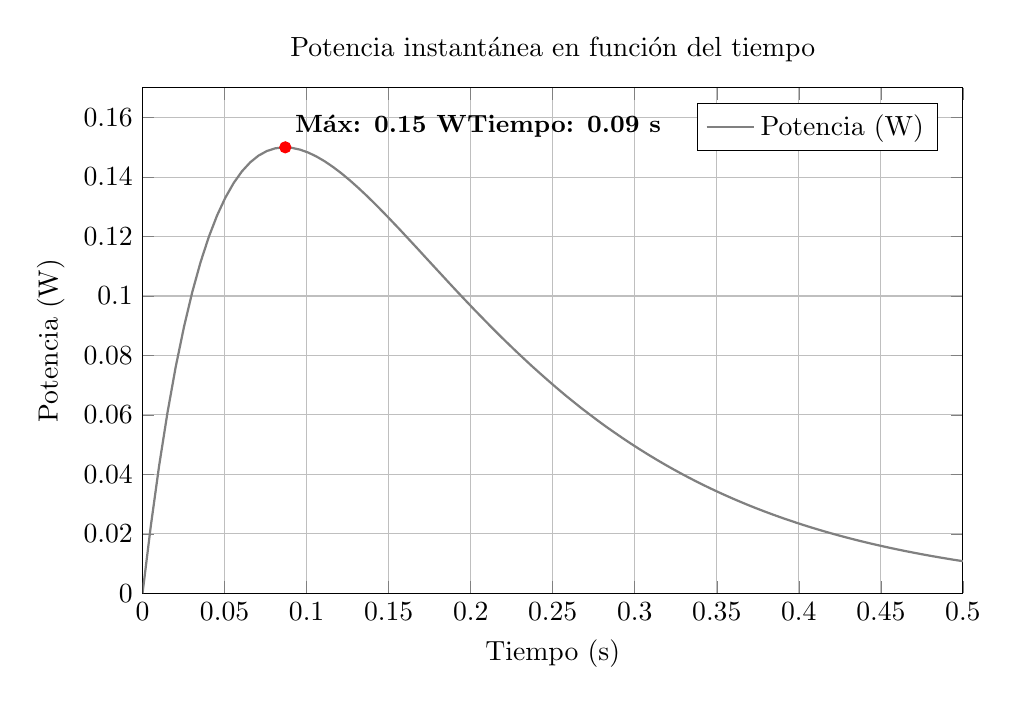
\begin{tikzpicture}
            \begin{axis}[
                xlabel={Tiempo (s)},
                ylabel={Potencia (W)},
                title={Potencia instantánea en función del tiempo},
                legend pos=north east,
                grid=major,
                ymin=0, ymax=0.17,
                xmin=0, xmax=0.5,
                width=12cm, height=8cm,
                axis background/.style={fill=white}, % Fondo blanco
                tick label style={/pgf/number format/fixed}, % Evita notación científica
            ]
        
            % Definimos la función de potencia
            \addplot[color=gray, thick, domain=0:0.5, samples=100] 
                {0.6 * (1 - exp(-8*x)) * exp(-8*x)};
            \addlegendentry{Potencia (W)}
        
            % Punto máximo de la potencia
            \draw[red, fill=red] (axis cs:0.087,0.15) circle (2pt);
            \node[anchor=south west] at (axis cs:0.087,0.15) 
                {\small \textbf{Máx: 0.15 W}\\ \small \textbf{Tiempo: 0.09 s}};
        
            \end{axis}
        \end{tikzpicture}
    \end{solution}
    %%%%%%%%%%%%%%%%%%%%%%%%%%%
    \question  Para el circuito de la figura 1:

    \begin{itemize}
        \item El valor de R2 respecto a R1 que maximiza la potencia disipada en R2.
        \item Qué ocurre con la potencia si el valor de R2 es muy alto (Aprox. a $\infty$).
        \item Qué ocurre con la potencia si el valor de R2 es muy bajo (Aprox. a 0).
    \end{itemize}
    \begin{center}
        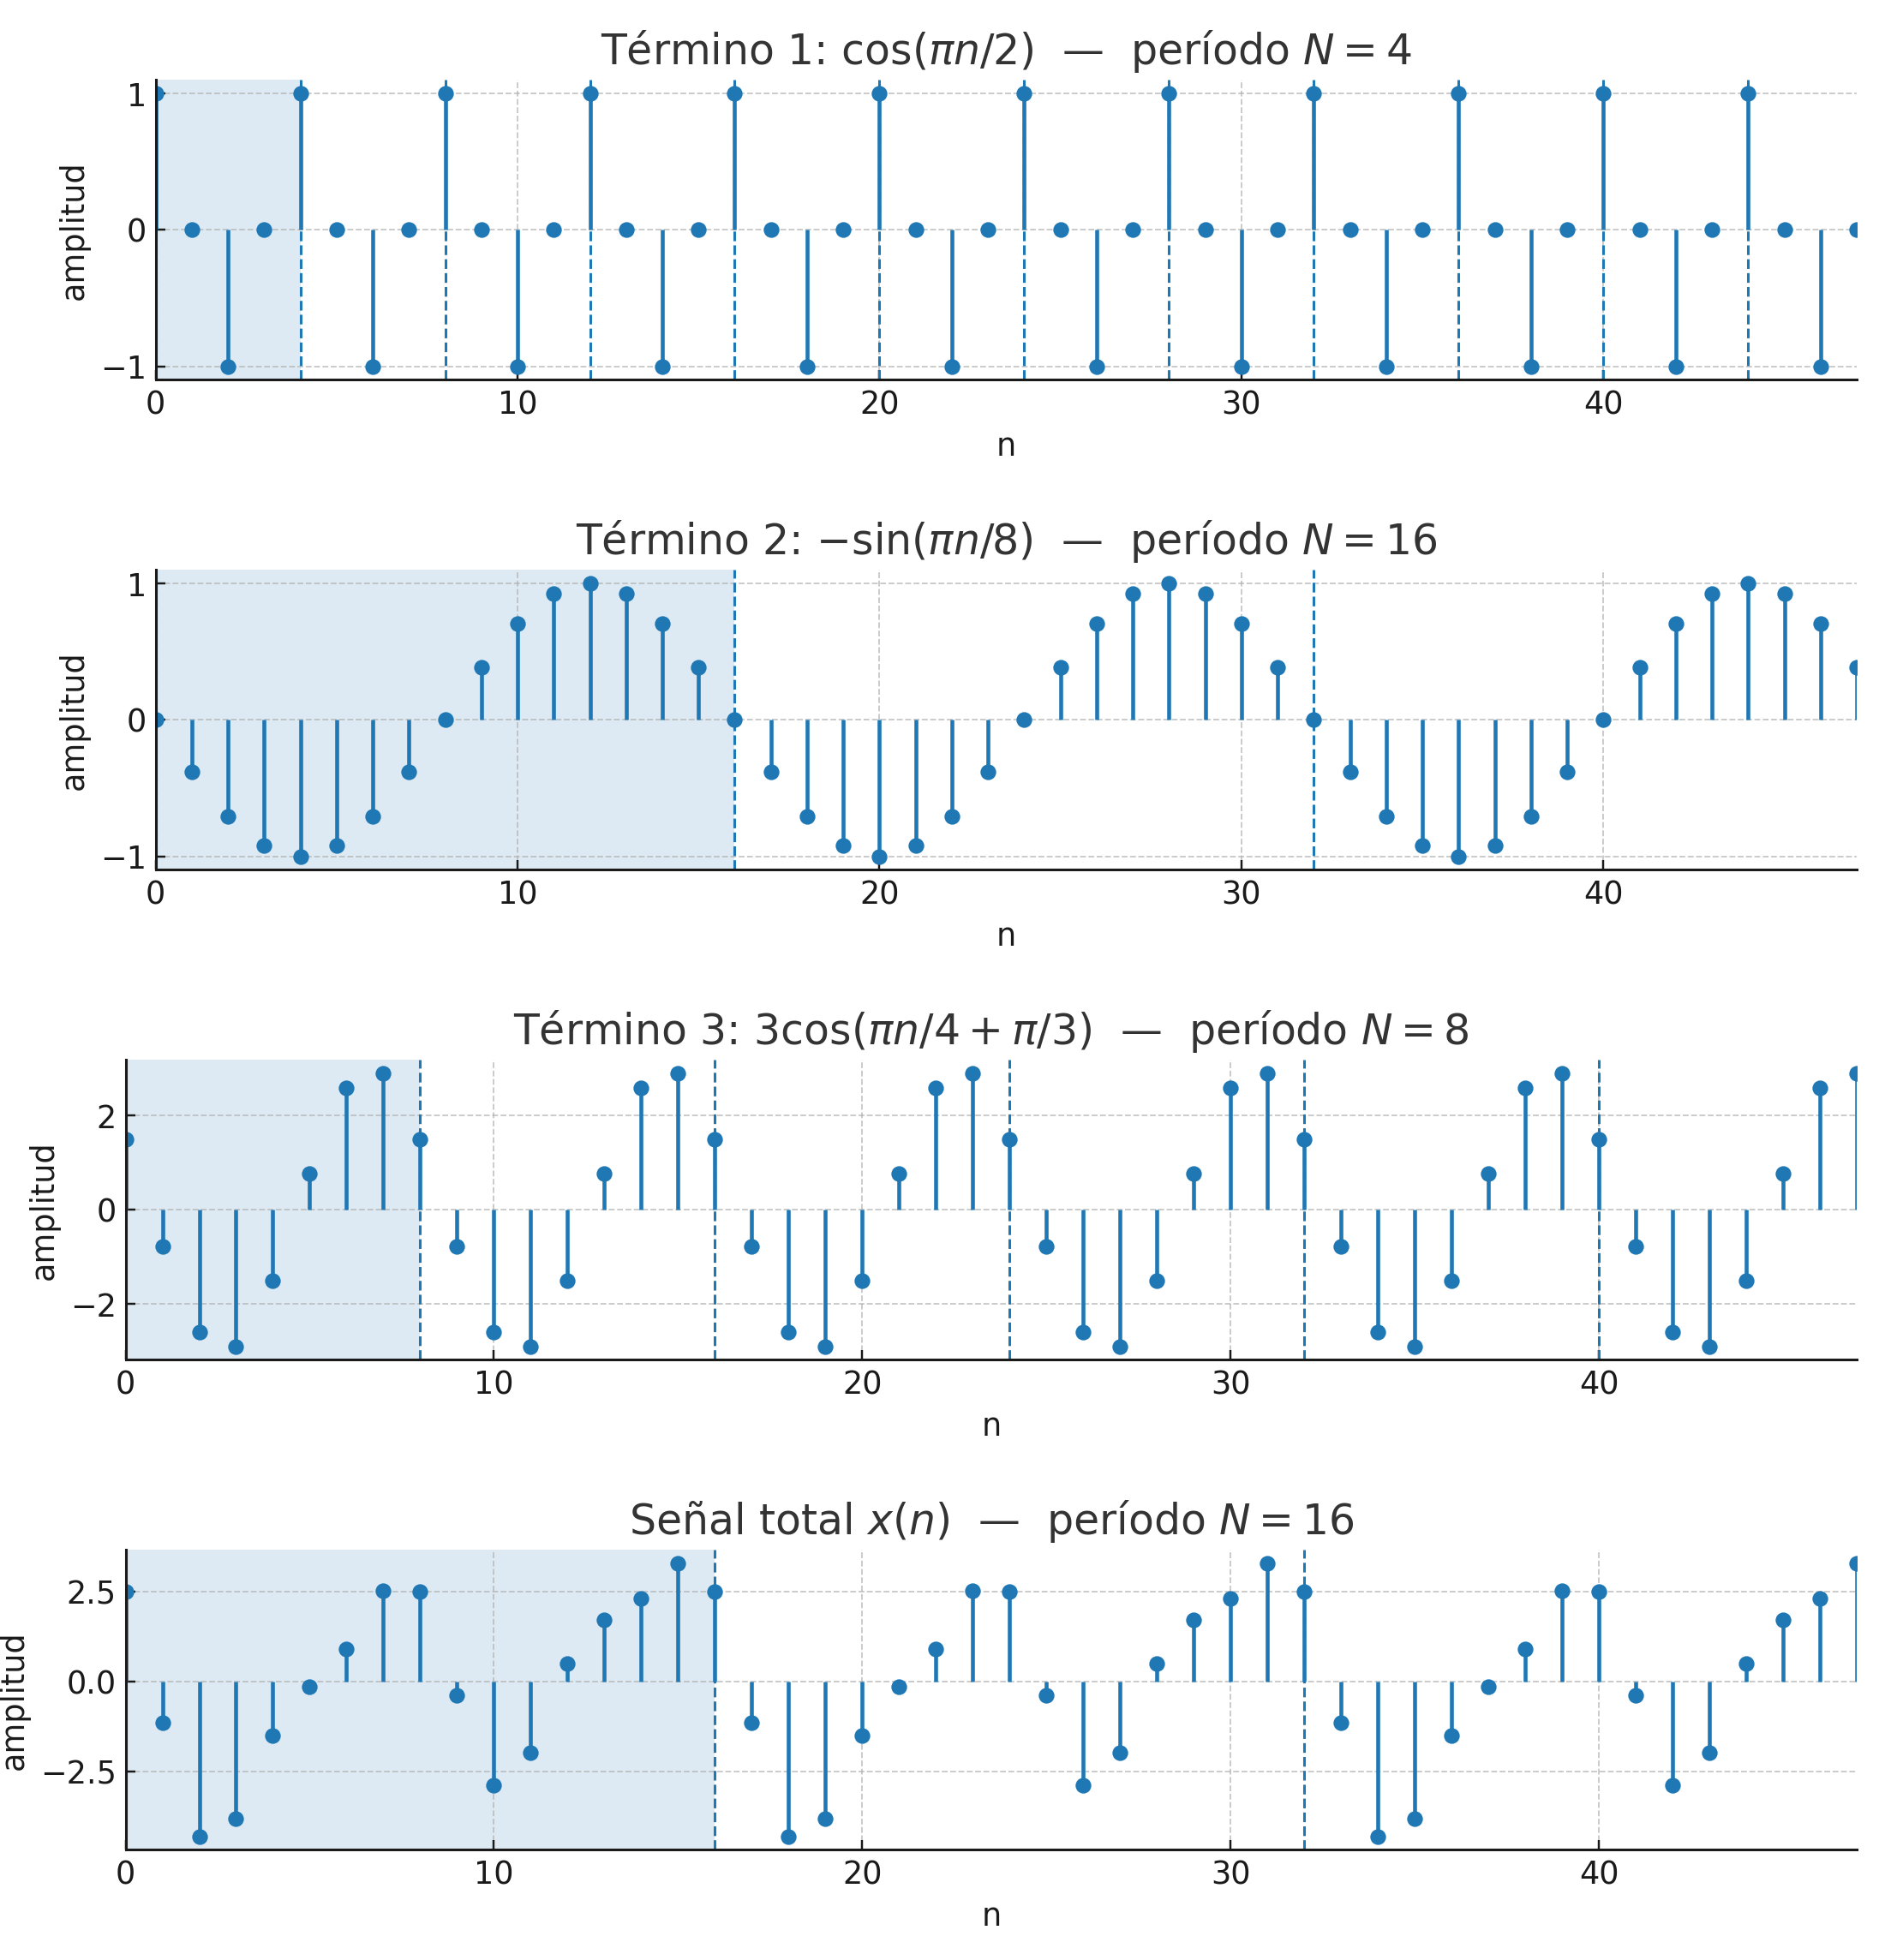
\includegraphics[width=0.3\textwidth]{Auxiliar_1_1}
        \captionof{figure}{Esquema del circuito}
    \end{center}
    %%%%%%%%%%%%%%%%%%%%%%%%%%%
    \begin{solution}
        \begin{itemize}
            \item Se busca obtener el valor de $R_2$ respecto a $R_{1}$ que maximiza la potencia disipada en $R_2$, por lo tanto:
            \begin{align}
            V - V_{R1} - V_{R2} &= 0\\
            V &= V_{R1} + V_{R2}\\
            V &= R_{1} \cdot I_{1} + R_{2} \cdot I_{1}\\
            I_{1} &= \frac{V}{R_{1} + R_{2}}
            \end{align}
            Luego reemplazando sobre la potencia disipada en $R_{2}$:
            \begin{align}
                P_{R2} &= V_{R2} \cdot I_{1}\\
                &= R_{2} \cdot I_{1}^{2}\\
                &= R_{2} \cdot \left( \frac{V}{R_{1} + R_{2}} \right)^{2}
            \end{align}
            Para cumplir la condicion de maximo se deriva respecto a $R_{2}$ y se iguala a 0, tal que:
            \begin{align}
                \frac{dP_{R2}}{dR_{2}} &= 0\\
                \frac{d}{dR_{2}} \left( R_{2} \cdot \left( \frac{V}{R_{1} + R_{2}} \right)^{2} \right) &= 0\\
                \frac{1}{(R_{1} + R_{2})^{2}} - \frac{2R_{2}}{(R_{1} + R_{2})^{3}} &= 0\\
                \frac{1}{(R_{1} + R_{2})^{2}} &= \frac{2R_{2}}{(R_{1} + R_{2})^{3}}\\
                1 &= \frac{2R_{2}}{(R_{1}+R_{2})}\\
                R_{1} + R_{2} &= 2R_{2}\\
                R_{1} &= R_{2}
            \end{align}
            De esta manera se obtiene que el valor de $R_{2}$ respecto a $R_{1}$ que maximiza la potencia disipada en $R_{2}$ es $R_{1} = R_{2}$.
            \item Analizando este caso en diferentes aspectos, tenemos que:
            \begin{equation}
                lim_{R_{2} \to \infty} (P_{R2}) = \frac{R_{2 \cdot V^{2}}}{(R_{1} + R_{2})^{2}} = \frac{\frac{1}{R_{2}} \cdot V^{2}}{(\frac{R_{1}}{(R_{2})^{2}} + 1)^{2}} = 0
            \end{equation}
            Por otro lado el voltaje se tendra que:
            \begin{equation}
                lim_{R_{2} \to \infty} (V_{R2}) = R_{2} \cdot I_{1} = R_{2}\left( \frac{V}{R_{1} + R_{2}} \right) = \frac{V}{\left( \frac{1}{R_{2}+1}\right)} = V
            \end{equation}
        Por ultimo la corriente se tendra que:
        \begin{equation}
            lim_{R_{2} \to \infty} (I_{1}) = \frac{V}{R_{1} + R_{2}} = 0
        \end{equation}
        Este fenomeno es conocido como un circuito abierto, puede entenderse como que la resistencia tiende a infinito y por tanto no permite circular corriente, por lo tanto no se disipa potencia.
        \begin{center}
            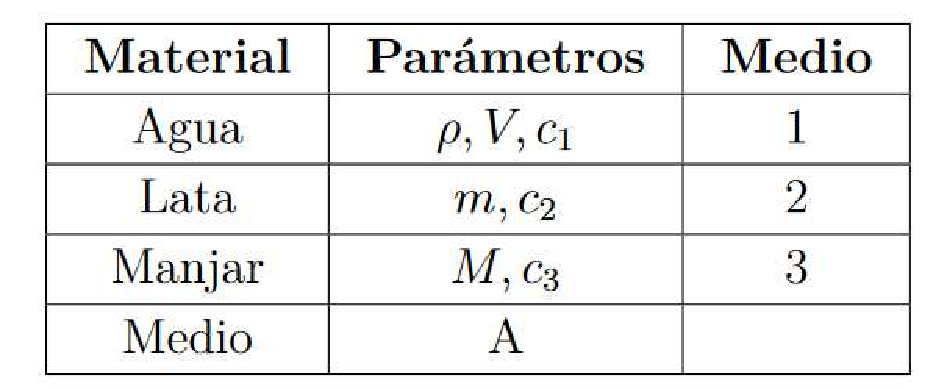
\includegraphics[width=0.3\textwidth]{Auxiliar_1_4}
            \captionof{figure}{Esquema del circuito abierto}
        \end{center}
        \item Por otro lado sea el caso que $R_{2}$ tiende a 0, se tiene que en base al mismo analisis:
        \begin{equation}
            lim_{R_{2} \to 0} (P_{R2}) = \frac{R_{2 \cdot V^{2}}}{(R_{1} + R_{2})^{2}} = \frac{0 \cdot V^{2}}{(R_{1})^{2}} = 0
        \end{equation}
        Por otro lado el voltaje se tendra que:
        \begin{equation}
            lim_{R_{2} \to 0} (V_{R2}) = R_{2} \cdot I_{1} = R_{2}\left( \frac{V}{R_{1} + R_{2}} \right) = 0
        \end{equation}
        Por ultimo la corriente se tendra que:
        \begin{equation}
            lim_{R_{2} \to 0} (I_{1}) = \frac{V}{R_{1} + R_{2}} = \frac{V}{R_{1}} = \frac{V}{R_{1}}
        \end{equation}
        Este fenomeno es conocido como un corto circuito, puede entenderse como que la resistencia tiende a 0 y por tanto no permite caida de voltaje, por lo tanto no se disipa potencia.
        \begin{center}
            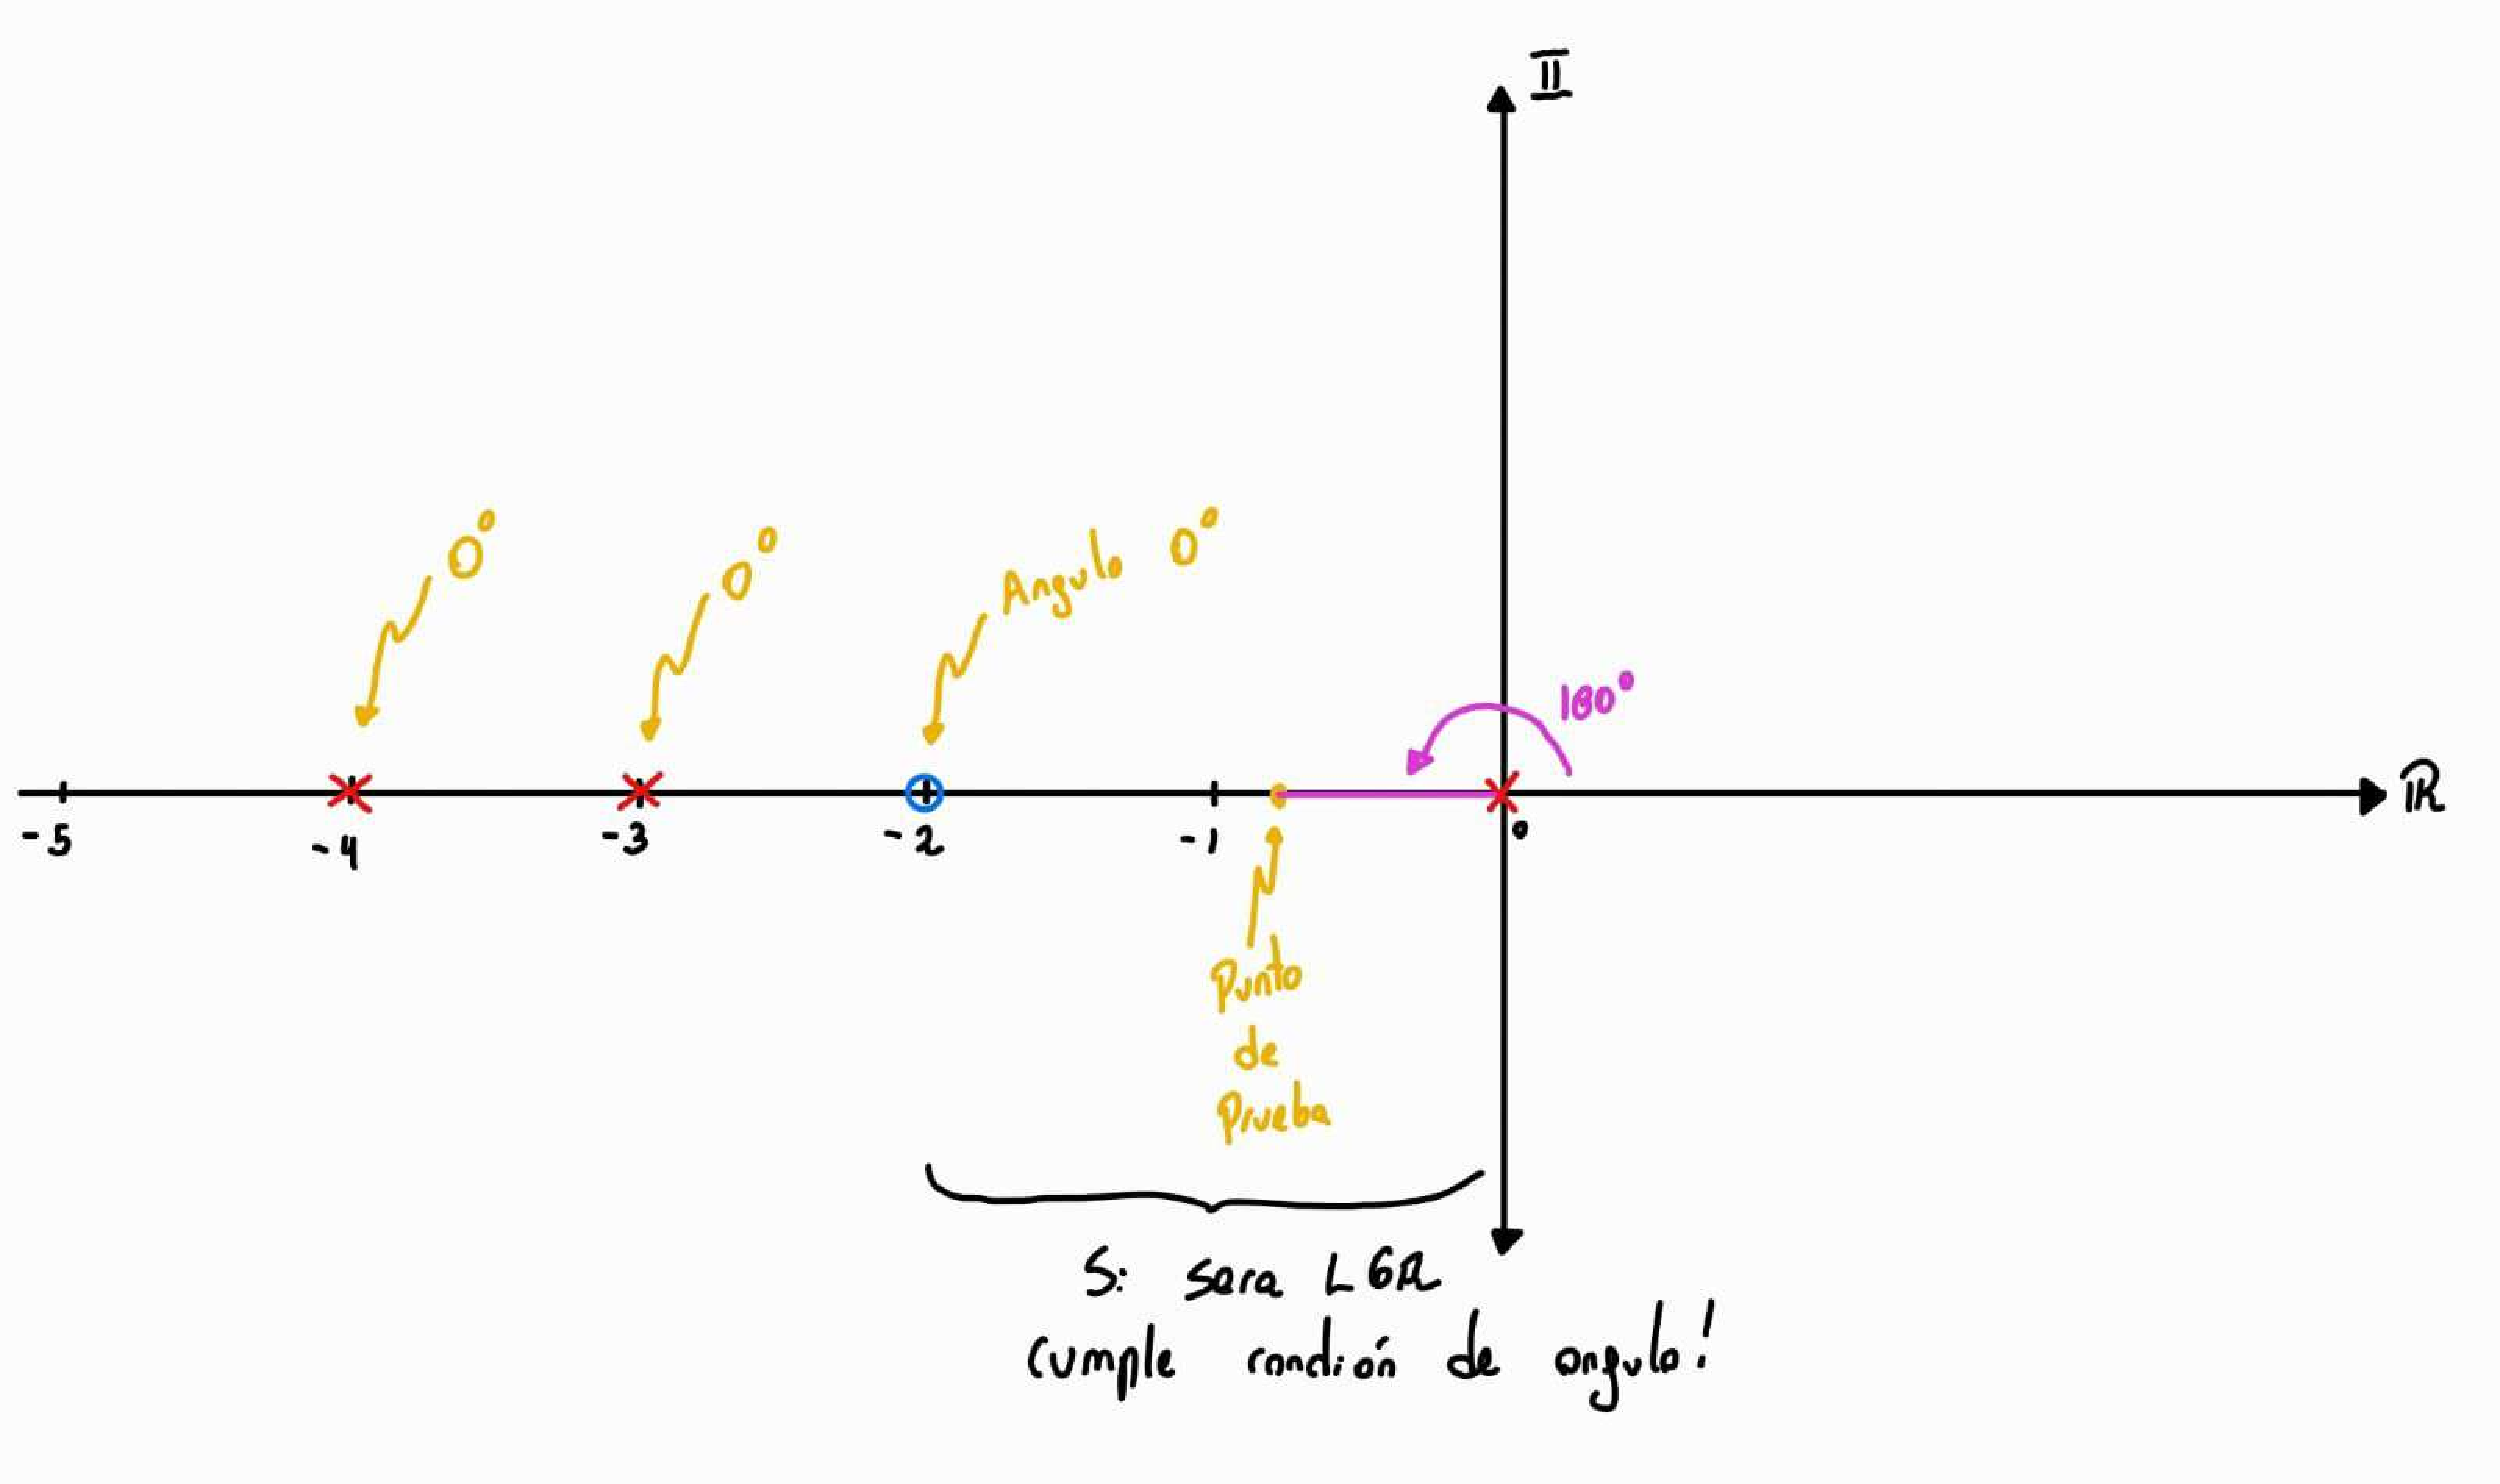
\includegraphics[width=0.3\textwidth]{Auxiliar_1_5}
            \captionof{figure}{Esquema del circuito cerrado para $R_{2}$}
        \end{center}
        Estos dos conceptos es super importante entenderlos y no confundirlos.
    \end{itemize}
    \end{solution}
%%%%%%%%%%%%%%%%%%%%%%%%%%%
\question  
\begin{enumerate}
    En base a la figura del enunciado:
    \item Asigne referencias a cada elemento.
    \item Use LVK para encontrar el voltaje en cada resistencia.
    \item Use la ley de Ohm para encontrar la corriente en cada resistencia.
    \item Use LCK para encontrar la corriente que pasa a través de cada fuente de voltaje.
\end{enumerate}
\begin{center}
    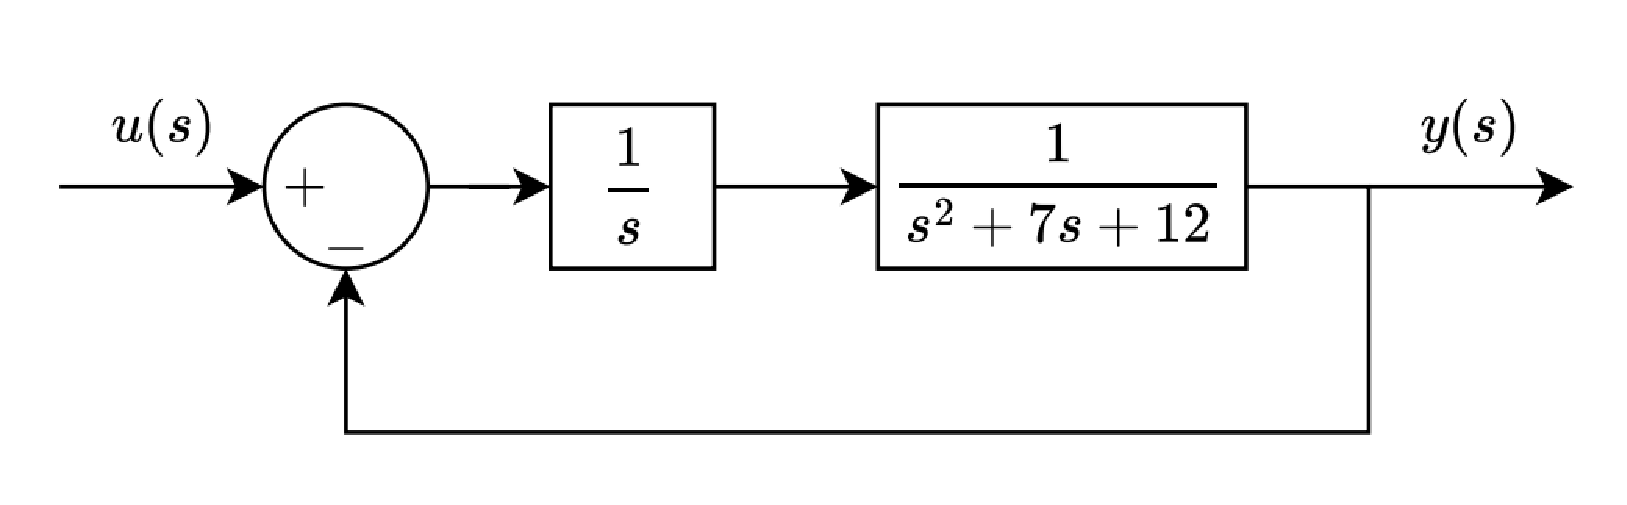
\includegraphics[width=0.5\textwidth]{Auxiliar_1_2}
    \captionof{figure}{Esquema del circuito}
\end{center}
%%%%%%%%%%%%%%%%%%%%%%%%%%%
\begin{solution}
   \begin{enumerate}
    \item Las asignaciones de referencias son arbitrarias y propias de quien las plantee, el unico requerimiento es que se mantenga la consistencia en el analisis, en este caso particular:
    \begin{center}
        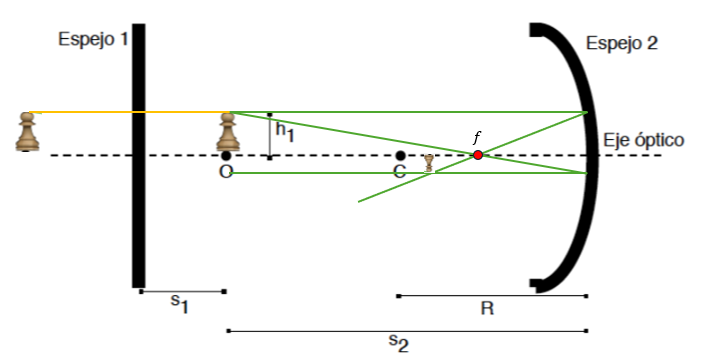
\includegraphics[width=0.5\textwidth]{Auxiliar_1_6}
        \captionof{figure}{Esquema del circuito}
    \end{center}
    \item Se busca obtener el voltaje en cada resistencia, por lo tanto se plantea LVK en cada malla:
    \begin{center}
        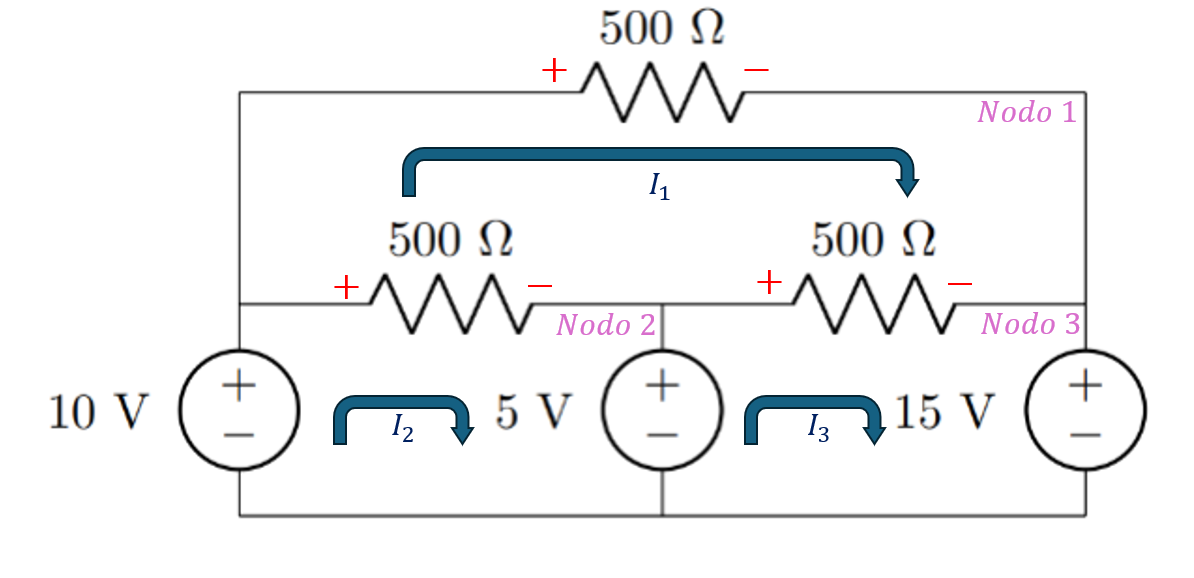
\includegraphics[width=0.6\textwidth]{Auxiliar_1_7}
        \captionof{figure}{Esquema del circuito con todas las referencias}
    \end{center}
    Luego para cada nodo tenemos lo siguiente:
    \begin{align}
        \sum_{\text{Nodo 1}} V_{n} &= V_{1} - V_{2} - V_{3} = 0\\
        V_{1} &= V_{2} + V_{3}
    \end{align}
    \begin{align}
        \sum_{\text{Nodo 2}} V_{n} &= 5[v] - 10[v] + V_{2} = 0\\
        V_{2} &= 5[v]
    \end{align}
    \begin{align}
        \sum_{\text{Nodo 3}} V_{n} &= 15[v] - 5 + V_{3} = 0\\
        V_{3} &= -10[v]
    \end{align}
    Con lo que se puede obtener el voltaje $V_{1}$ tal que:
    \begin{equation}
        V_{1} = 5[v] - 10[v] = -5[v]
    \end{equation}
    \item Luego mediante la ley de Ohm se puede obtener la corriente en cada resistencia, tal que:
    \begin{align}
   
    \end{enumerate}

\end{solution}
%%%%%%%%%%%%%%%%%%%%%%%%%%%
\question \begin{enumerate}
    \item Identifique todos los nodos.
    \item Simplifique el circuito lo que más pueda y luego asigne referencia de signos.
    \item Plantee todas las ecuaciones de malla (incluyendo la ec. de malla exterior) y demuestre que hay una ecuación innecesaria para el análisis.
    \item Calcule las corrientes incógnitas del método de mallas considerando que todas las resistencias tienen el mismo valor.
\end{enumerate}
\begin{center}
    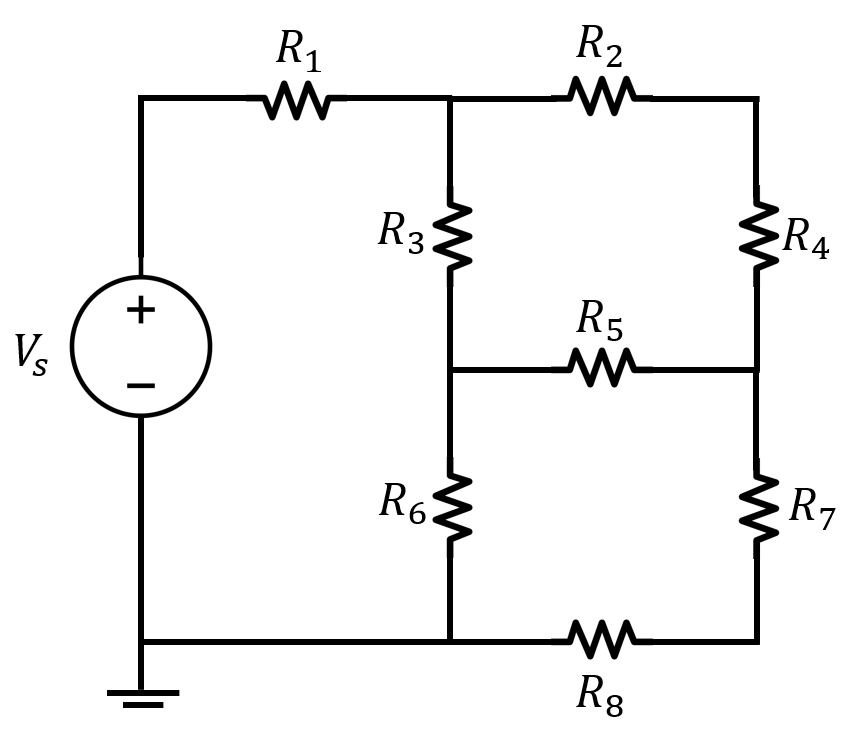
\includegraphics[width=0.4\textwidth]{Auxiliar_1_3}
    \captionof{figure}{Esquema del circuito}
\end{center}
\end{questions}
\newpage
%%%%%%%%%%%%%%%%%%%%%%%%%%%

\end{document}